\documentclass[a4paper,12pt]{article}
\usepackage[utf8]{inputenc}
\usepackage[spanish]{babel}
\usepackage{tikz}
\usepackage{geometry}
\usepackage{setspace}
\usepackage{titlesec}
%\usepackage{lmodern}
\usepackage{multicol}
\usepackage{fancyhdr}
\usepackage{graphicx}
%\usepackage{helvet}
%\usepackage{mathptmx}
\usepackage{amsmath}       
\usepackage{amssymb}      
\usepackage{adjustbox}     
\usepackage{lastpage}
\usepackage{pgfplots}
\pgfplotsset{compat=1.17}
\usepackage{amsmath}
\usepackage{minted}
\usepackage{wrapfig}

\usepackage{tabularx}
\usepackage{qrcode}
\usepackage{tikz}
\usetikzlibrary{matrix, fit, positioning}



\usepackage{hyperref}
\usepackage{booktabs}
\usepackage{array}
\usepackage{float}
\usepackage{longtable}  

\renewcommand{\arraystretch}{1.4}
\setlength{\tabcolsep}{8pt} 

\setlength{\footskip}{25pt}
%---------------------------python
\usepackage[T1]{fontenc}
\usepackage[utf8]{inputenc}

\usepackage{listings}
\usepackage{xcolor}

\lstdefinestyle{pythonstyle}{
	language=Python,
	basicstyle=\ttfamily\small,
	keywordstyle=\color{blue},
	stringstyle=\color{red},
	commentstyle=\color{gray},
	numbers=left,
	numberstyle=\tiny\color{gray},
	stepnumber=1,
	numbersep=5pt,
	showspaces=false,
	showstringspaces=false,
	breaklines=true,
	frame=single,
	tabsize=4
}



%-------------------------------Consola
\usepackage{listings}
\usepackage{xcolor}

\lstdefinestyle{consola}{
	backgroundcolor=\color{black!5},
	basicstyle=\ttfamily,
	frame=single,
	keywordstyle=\color{blue},
	commentstyle=\color{gray},
	showstringspaces=false
}

%Plano Z y Z^2

\usepackage[utf8]{inputenc}
\usepackage{amsmath, amssymb}
\usepackage{pgfplots}
\pgfplotsset{compat=1.18}
\usepackage{geometry}
\geometry{a4paper, margin=2.5cm}


\geometry{top=2.5cm, bottom=2.5cm, left=2.5cm, right=1.5cm}

% Estilo de página
\pagestyle{fancy}
\fancypagestyle{miestilo}{
	\fancyhf{} % Limpia encabezado y pie
	
	% Encabezado izquierda: logo
	\fancyhead[L]{%
		\vspace{0.1cm}
		\adjustbox{valign=c,scale=0.15}{%
			\begin{tikzpicture}
				\clip (-3,-2.8) rectangle (3,2.8);
				\draw[black,line width=0.8cm] (-2.3,0)--(2.3,0);
				\draw[black,line width=0.8cm] (0,-2.85)--(0,2.85);
				\draw[black,line width=0.87cm] (0,2.8) circle(2);
				\draw[black,line width=0.87cm] (0,-2.8) circle(2);
			\end{tikzpicture}
		}%
	}
	
	% Encabezado centro: título
	\fancyhead[C]{\textbf{Técnicas Digitales 1   
	}}
	
	% Encabezado derecha: TP y año debajo
	\fancyhead[R]{%
		TP de Laboratorio N°1 \\ 2026
	}
	
	% Línea en el encabezado y pie
	\renewcommand{\headrulewidth}{0.4pt}
	\renewcommand{\footrulewidth}{0.4pt}
	
	% Pie de página derecha: Página X de Y
	\fancyfoot[R]{Página \thepage\ de \pageref{LastPage}}
}


\begin{document}
	
	% --------- PORTADA ---------
	\pagestyle{empty}
	\begin{center}
		\textbf{\LARGE UNIVERSIDAD TECNOLÓGICA NACIONAL}\\[0.2cm]
		\textbf{\Large FACULTAD REGIONAL CÓRDOBA}\\[0.5cm]
		\textbf{\large INGENIERÍA ELECTRÓNICA}\\[1.5cm]
		
		\begin{tikzpicture}
			\clip (-3,-2.8) rectangle (3,2.8);
			\draw[black,line width=0.8cm] (-2.3,0)--(2.3,0);
			\draw[black,line width=0.8cm] (0,-2.85)--(0,2.85);
			\draw[black,line width=0.87cm] (0,2.8) circle(2);
			\draw[black,line width=0.87cm] (0,-2.8) circle(2);
		\end{tikzpicture}
		
		\vspace{1cm}
		\textbf{\huge Técnicas Digitales 1   
		}\\[0.5cm]
		\rule{\textwidth}{0.4pt}\\[0.3cm]
		\textbf{\Huge Trabajo Práctico de Laboratorio N°1
		}\\[0.3cm]
		{\large Álgebra de Boole y Circuitos Combinacionales}\\[0.3cm]
		\rule{\textwidth}{0.4pt}\\[1.5cm]
	\end{center}
	
	\begin{flushleft}
		\begin{tabular}{@{}ll}
			DOCENTES     & : Esp.Ing. Marcelo Casasnovas\\ 
			& \ \  Ing Florencia Belén Molla JTP \\[0.2cm]
			CÁTEDRA      & :  Técnicas Digitales 1   \\[0.2cm]
			CURSO        & : 3R4 \\[0.2cm]
			ALUMNO      & :
			\begin{tabular}[t]{@{}l l}
				Gonza Elías Noel Imanol           & 87669 \\ 
			\end{tabular}
		\end{tabular}
	\end{flushleft}
	
	\vfill
	\begin{center}
		\textbf{CÓRDOBA, ARGENTINA}\\
		\textbf{2026}
	\end{center}
	\pagestyle{empty}
	% --------- CAMBIO DE ESTILO ---------
	\newpage
	\pagenumbering{arabic}
	\pagestyle{miestilo}
	% --------- CONTENIDO ---------
	\tableofcontents
	\newpage
	
	
	\section{Introducción}
	
	En este laboratorio vamos a aplicar los conceptos aprendidos en las unidades 1 y 2 de la materia. En el primer punto se diseñará un conversor que transforma un número en código BCD a su equivalente en Exceso 3. De aquí desarrollaremos la tabla de verdad y su correspondiente mapa de Karnaugh para poder simplificar las funciones. Además, se llevará a la práctica utilizando el simulador Falstad y luego lo implementaremos en una protoboard junto con el MiniLab.
	
	Para el siguiente ejercicio haremos un comparador binario que evaluará tres situaciones distintas: determinar si un número $A$ es mayor que un número $B$, si es menor o si ambos son iguales. Para esto, se utilizarán tres salidas que indicarán el resultado según el orden establecido. Al igual que en el caso anterior, se realizará la simplificación de la función utilizando el mapa de Karnaugh y se llevará a la práctica utilizando un simulador y una protoboard.
	
	\section{Teoría de los Códigos BCD y Exceso 3}
	
	\subsection{Código BCD}
	
	En informática, BCD es un código que se utiliza para representar números decimales en código binario. En BCD, o decimal codificado en binario, cada número decimal del $0$ al $9$ es representado por su equivalente en binario en 4 bits.
	
	\subsection{Código Exceso 3}
	
	El código Exceso 3 para un número decimal se obtiene de la misma forma que el BCD, excepto que se suma el número $3$ a cada dígito decimal antes de modificarlo en binario.
	
	Por ejemplo, para codificar el número decimal $4$ en código Exceso 3, primero debemos sumar $3$:
	
	\[
	4 + 3 = 7
	\]
	
	Luego, el número $7$ se codifica en su equivalente binario de 4 bits:
	
	\[
	7_{10} = 0111_2
	\]
	
	Por lo tanto, el número decimal $4$ en código Exceso 3 se representa como:
	
	\[
	4_{10} \rightarrow 0111_2
	\]
	
	\section{Conversor de Código BCD a Exceso 3: Diseño, Simplificación, Simulación e Implementación}
	
	Este conversor cuenta con 4 entradas representadas por interruptores On-Off, donde cada interruptor codifica un dígito binario. Por ejemplo, si todos los interruptores están en posición Off, la entrada será $0000$ en binario.
	
	La salida del conversor se representa mediante 4 LEDs, los cuales indican el número en código Exceso 3. Por ejemplo, si la entrada es $0000$, correspondiente al decimal $0$ en BCD, la salida será $0011$, equivalente al decimal $3$ en Exceso 3.
	
	\[
	0000_{BCD} \rightarrow 0011_{XS3}
	\]
	
	
	\subsection{Diseño}
	
	Así será el diagrama para empezar a tener una idea de cómo será el diseño. Las entradas $A0$, $B0$, $C0$ y $D0$ serán representadas mediante interruptores, mientras que las salidas $A1$, $B1$, $C1$ y $D1$ serán representadas mediante LEDs.
	
	\begin{figure}[h]
		\centering
		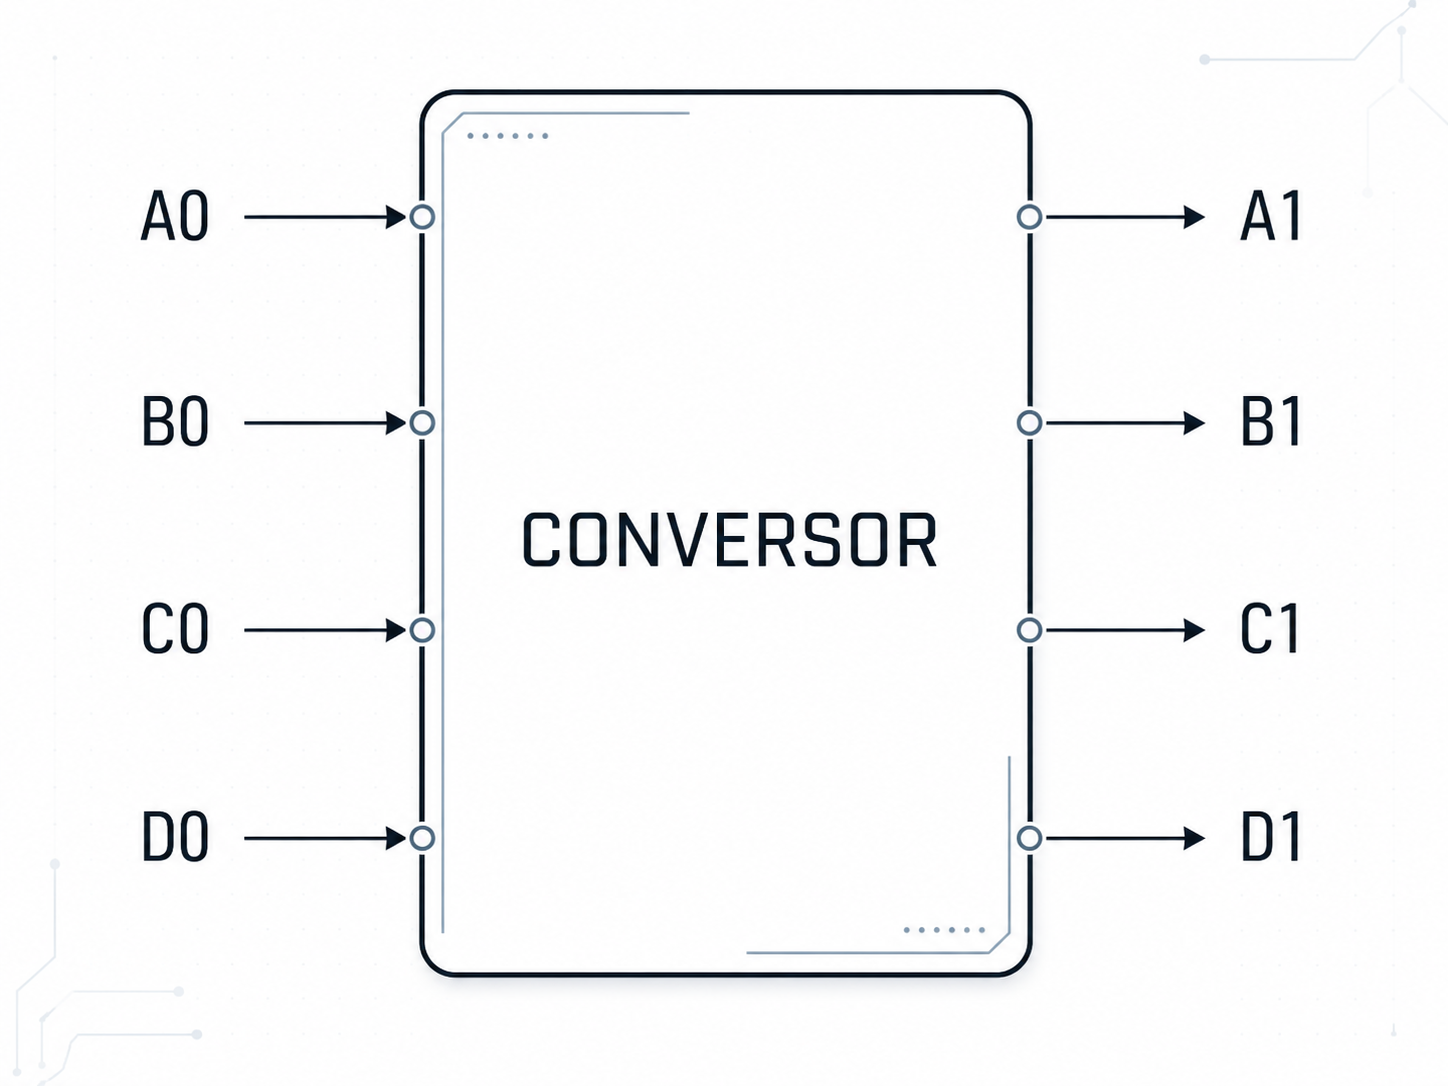
\includegraphics[width=0.4\textwidth]{Conversor.png}
		\caption{Diagrama general del conversor BCD a Exceso 3.}
		\label{fig:conversor_bcd_exceso3}
	\end{figure}
	
	\subsection{Tabla de Verdad}
	
	En la siguiente tabla se muestran las combinaciones de 4 bits tanto en BCD como en Exceso 3. También se indican las funciones de salida $A1$, $B1$, $C1$ y $D1$, las cuales tomarán los valores $1$ o $0$ dependiendo de las entradas BCD $A0$, $B0$, $C0$ y $D0$.
	
	\begin{table}[H]
		\centering
		\begin{tabular}{|c|c|c|c|}
			\hline
			\textbf{Decimal} & \textbf{Binario} & \textbf{BCD} & \textbf{Exceso 3} \\
			\hline
			0 & 0000 & 0000 & 0011 \\
			1 & 0001 & 0001 & 0100 \\
			2 & 0010 & 0010 & 0101 \\
			3 & 0011 & 0011 & 0110 \\
			4 & 0100 & 0100 & 0111 \\
			5 & 0101 & 0101 & 1000 \\
			6 & 0110 & 0110 & 1001 \\
			7 & 0111 & 0111 & 1010 \\
			8 & 1000 & 1000 & 1011 \\
			9 & 1001 & 1001 & 1100 \\
			\hline
			\multicolumn{2}{|c|}{} & $A0\ B0\ C0\ D0$ & $A1\ B1\ C1\ D1$ \\
			\hline
		\end{tabular}
		\caption{Tabla de conversión de BCD a Exceso 3.}
		\label{tab:bcd_exceso3}
	\end{table}
	
	\subsection{Tabla de Salidas}
	
	A partir de la tabla de verdad anterior, se obtienen las salidas correspondientes del conversor:
	
	\begin{table}[h]
		\centering
		\begin{tabular}{|c|c|c|c|}
			\hline
			\textbf{$A1$} & \textbf{$B1$} & \textbf{$C1$} & \textbf{$D1$} \\
			\hline
			0 & 0 & 1 & 1 \\
			0 & 1 & 0 & 0 \\
			0 & 1 & 0 & 1 \\
			0 & 1 & 1 & 0 \\
			0 & 1 & 1 & 1 \\
			1 & 0 & 0 & 0 \\
			1 & 0 & 0 & 1 \\
			1 & 0 & 1 & 0 \\
			1 & 0 & 1 & 1 \\
			1 & 1 & 0 & 0 \\
			\hline
		\end{tabular}
		\caption{Estados de salida $A1$, $B1$, $C1$ y $D1$ para cada entrada BCD.}
		\label{tab:salidas_exceso3}
	\end{table}
	
	
	\subsection{Simplificación}
	
	Luego de armar los mapas de Karnaugh, llegamos a la simplificación de las siguientes funciones $A_1$, $B_1$, $C_1$ y $D_1$.
	
	\bigskip
	
	\tikzset{
		kmap/.style={
			matrix of nodes,
			nodes={
				draw,
				minimum width=0.95cm,
				minimum height=0.72cm,
				anchor=center,
				font=\small
			},
			column sep=-\pgflinewidth,
			row sep=-\pgflinewidth
		},
		grupo/.style={
			rounded corners=1pt,
			very thick,
			inner sep=2pt
		}
	}
	
	%========================================================
	% A1
	%========================================================
	\noindent
	\begin{minipage}{0.62\textwidth}
		\[
		\begin{tikzpicture}
			
			\matrix (K) [kmap] {
				& 00 & 01 & 11 & 10 \\
				00 & 0 & 0 & 0 & 0 \\
				01 & 0 & 1 & 1 & 1 \\
				11 & X & X & X & X \\
				10 & 1 & 1 & X & X \\
			};
			
		\node[font=\scriptsize, above left=0.05cm and -0.15cm of K-2-1.north east] {$A_0B_0$};
		\node[font=\scriptsize, above right=0.02cm and -0.05cm of K-1-2.north west] {$C_0D_0$};
		
			
			\draw (K-2-1.north west) -- (K-1-2.south west);
			
			\node[draw=blue, grupo, fit=(K-4-2)(K-5-5)] {};
			\node[draw=green!60!black, grupo, fit=(K-3-3)(K-3-4)(K-4-3)(K-4-4)] {};
			\node[draw=red, grupo, fit=(K-3-4)(K-3-5)(K-4-4)(K-4-5)] {};
			
		\end{tikzpicture}
		\]
	\end{minipage}
	\hfill
	\begin{minipage}{0.33\textwidth}
		\[
		A_1 = A_0 + B_0(C_0 + D_0)
		\]
	\end{minipage}
	
	\vspace{0.35cm}
	
	%========================================================
	% B1
	%========================================================
	\noindent
	\begin{minipage}{0.62\textwidth}
		\[
		\begin{tikzpicture}
			
			\matrix (K) [kmap] {
				& 00 & 01 & 11 & 10 \\
				00 & 0 & 1 & 1 & 1 \\
				01 & 1 & 0 & 0 & 0 \\
				11 & X & X & X & X \\
				10 & 0 & 1 & X & X \\
			};
			
			\node[font=\scriptsize, above left=0.05cm and -0.15cm of K-2-1.north east] {$A_0B_0$};
			\node[font=\scriptsize, above right=0.02cm and -0.05cm of K-1-2.north west] {$C_0D_0$};
			
			
			\draw (K-2-1.north west) -- (K-1-2.south west);
			
			% Grupo azul
			\node[draw=blue, grupo, fit=(K-2-3)(K-2-4)] {};
			\node[draw=blue, grupo, fit=(K-5-3)(K-5-4)] {};
			
			% Grupo verde
			\node[draw=green!60!black, grupo, fit=(K-3-2)(K-4-2)] {};
			
			% Grupo rojo
			\node[draw=red, grupo, fit=(K-2-4)(K-2-5)] {};
			\node[draw=red, grupo, fit=(K-5-4)(K-5-5)] {};
			
		\end{tikzpicture}
		\]
	\end{minipage}
	\hfill
	\begin{minipage}{0.33\textwidth}
		\[
		B_1 = B_0D_0'C_0' + B_0'(D_0 + C_0)
		\]
	\end{minipage}
	
	\vspace{0.35cm}
	
	%========================================================
	% C1
	%========================================================
	\noindent
	\begin{minipage}{0.62\textwidth}
		\[
		\begin{tikzpicture}
			
			\matrix (K) [kmap] {
				& 00 & 01 & 11 & 10 \\
				00 & 1 & 0 & 1 & 0 \\
				01 & 1 & 0 & 1 & 0 \\
				11 & X & X & X & X \\
				10 & 1 & 0 & X & X \\
			};
			
			\node[font=\scriptsize, above left=0.05cm and -0.15cm of K-2-1.north east] {$A_0B_0$};
			\node[font=\scriptsize, above right=0.02cm and -0.05cm of K-1-2.north west] {$C_0D_0$};
			
			
			\draw (K-2-1.north west) -- (K-1-2.south west);
			
			\node[draw=blue, grupo, fit=(K-2-2)(K-5-2)] {};
			\node[draw=red, grupo, fit=(K-2-4)(K-5-4)] {};
			
		\end{tikzpicture}
		\]
	\end{minipage}
	\hfill
	\begin{minipage}{0.33\textwidth}
		\[
		C_1 = C_0'D_0' + C_0D_0 =
		(C_0 \oplus D_0)'
		\]
	\end{minipage}
	
	\vspace{0.35cm}
	
	%========================================================
	% D1
	%========================================================
	\noindent
	\begin{minipage}{0.62\textwidth}
		\[
		\begin{tikzpicture}
			
			\matrix (K) [kmap] {
				& 00 & 01 & 11 & 10 \\
				00 & 1 & 0 & 0 & 1 \\
				01 & 1 & 0 & 0 & 1 \\
				11 & X & X & X & X \\
				10 & 1 & 0 & X & X \\
			};
			
			\node[font=\scriptsize, above left=0.05cm and -0.15cm of K-2-1.north east] {$A_0B_0$};
			\node[font=\scriptsize, above right=0.02cm and -0.05cm of K-1-2.north west] {$C_0D_0$};
			
	
		\draw[blue, very thick, rounded corners=1pt]
		([xshift=0.08cm,yshift=0.08cm]K-2-2.north west) --
		([xshift=-0.08cm,yshift=0.08cm]K-2-2.north east) --
		([xshift=-0.08cm,yshift=-0.08cm]K-5-2.south east) --
		([xshift=0.08cm,yshift=-0.08cm]K-5-2.south west);
		
	
		\draw[blue, very thick, rounded corners=1pt]
		([xshift=-0.08cm,yshift=0.08cm]K-2-5.north east) --
		([xshift=0.08cm,yshift=0.08cm]K-2-5.north west) --
		([xshift=0.08cm,yshift=-0.08cm]K-5-5.south west) --
		([xshift=-0.08cm,yshift=-0.08cm]K-5-5.south east);
		\end{tikzpicture}
		\]
	\end{minipage}
	\hfill
	\begin{minipage}{0.33\textwidth}
		\[
		D_1 = D_0'
		\]
	\end{minipage}
	
	
	
\subsection{Simulación}

Mediante el simulador online \textit{Falstad}, llevamos a cabo la implementación del circuito utilizando las compuertas correspondientes para comprobar su funcionamiento. Luego, verificamos su comportamiento con la tabla de verdad asociada.

\begin{figure}[H]
	\centering
	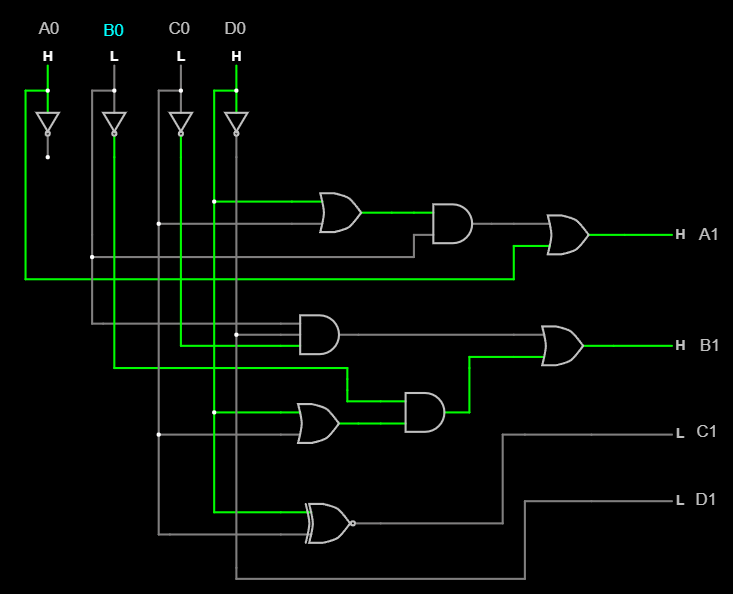
\includegraphics[width=0.7\textwidth]{Compuertas1.png}
	\caption{Simulación del conversor BCD a Exceso 3 en Falstad.}
	\label{fig:simulacion_falstad_bcd_exceso3}
\end{figure}

\begin{center}
	\href{\detokenize{https://www.falstad.com/circuit/circuitjs.html?ctz=DwYwlgTgBAZgvAIgIwKgFwM6IAwDpsEECsqYIiSeATAVQOx0DM2AHFQGwCcndqIARoiLZUAB0EIALI1QA3CENQBbTEICmAWiQoAfACgoUYAEkoAD0Ra67KJJZQrNpJMmp4CEVAwAbHLhJQABZgigD0+oYm5pYs2Lb2GrFQzq6wOKg+fgHBYRFGphbINnbJTi5u6V6+Hv6oOQgk4Qb50QicxfbtyeVpHhnVeNkhDQhNkQCCAHYAJq2MRFRQVJJxkuySSysVfWNGU7OFzBtESIvSiydU254A9rnNwPutSOyrBEt0ZwTXpJOIMrtgAB5aCFJDWJbLKCMGiQ1LuW73SIg56vKALez0C5UFg-KB3EaAlGFSRdSQvKDrVYvPEExp5YGgxCkmxUIg2djspbs2lIowAGVajniDnBNk8CLEFFGDMFhUSqwSSQl6UBcooHVKUBVO1lrTJnXFeNE0sBAFlWpzWVymNb2D9zZaVrYKbaXfbeiJHYVXvYiC4oG7-fDVQyLT7WJTnW6qQ6GQB3fWa9bxOMPRM+jYlFM0XGemXpp1LSNi4t5yWAjMakVaDppyJVhC1msU5Y6r0JoWt52ltv1oyNmFxKhQ+aLEch3WFkk550szbtgsNoVJEpaU6p-OVrsbtfacc8red+X77k2dfjljl0PTyynnH2MdLK-94CDhZn6Efh+vxvCte5puFbHpYgEAZGQ6-kKgFDrYXSQUet5SF0WJwTYCHAUhLxxIwLAbBo8F4VBJ4bg+oobrhk4dkhF7QnhDiEVRS4Dqi3QbBS5Iephy5gsUFLYe6xGIF0KRQGS3yITxwnFO8AkrIu26FKh8lobYEncSxJIwuiu7aS415TlJUh6SU5y2DCQnGWcelkhZkmaYgqEYtC2DHDillHKpbLFO0lneV5XJ2ApIEIP5QWfmsTGKRqcTsFe2qUi+9lvl2HLxbFSUaSlhyuZSnzxLFnyWeF7D5eFwbFUkwY6RcPRZX+SSiQqth2JZzX6RFrXJY2YUlGF6yvmYXYsJwDiMIwopohoMj5l4wzLKgaBqIg4zYAAOpMzHAEN8pdNNSAOKVop4hg82pEtiAAELrZtgI7aBY0TTiY0nWdi3LQgADCN1bfdCB0KN00TZQgMzZKc2OedH0ACI-XdrR0EQ9jrEQgbxaVATg6dkPvYg0NIBtv0I0Qo3+vYdAjeiJyvTj6AfZ9KDw4U1hZlQE0AxNkhEGDlTY6FUNXQTt0Mn91hPew7OcOOnA830EP87jCDjELW2NimVqlLFh71al6IBgJFXdaicSXFGNWWTmkYppcFvHBu6vazeRmm1SNWBgsbXdnEzaGzrJ42NVzZxQZ1GRAAGpMNxMkUhWLJ5pVXEbhSm9Vvp61FIUu86aexkn0lqXEXS2pZpuI4sRce3nbQ2G6FeJ5hwChOAED6EAA}}{Simulación 1 en Falstad}
\end{center}
Como podemos observar, para la combinación de entrada:

\[
A0 = 1,\quad B0 = 0,\quad C0 = 0,\quad D0 = 1
\]

en la salida se obtiene:

\[
A1 = 1,\quad B1 = 1,\quad C1 = 0,\quad D1 = 0
\]

Esto corresponde al número $9$ en BCD, ya que:

\[
1001_{BCD} = 9_{10}
\]

Al sumarle $3$ para obtener el código Exceso 3:

\[
9 + 3 = 12
\]

y el número $12$ en binario de 4 bits es:

\[
12_{10} = 1100_2
\]

Por lo tanto:

\[
1001_{BCD} \rightarrow 1100_{XS3}
\]

Esto coincide con lo indicado por la tabla de verdad del conversor. La simulación se puede consultar en el siguiente enlace:









\subsection{Implementación}

Una vez pasado el circuito a la simulación, ya podemos asegurarnos de que las funciones que resultan de aplicar el mapa de Karnaugh son correctas. Ahora, por último, vamos a llevar toda la teoría a la práctica, armando todo el circuito en una placa protoboard. Para ello, veremos su funcionamiento como lo mencionamos anteriormente.

Para tener una mayor facilidad en la implementación, vamos a llevar todo el circuito a compuertas NAND y NOT.

\subsubsection{Implementación para $A_1$}

Partimos de la función simplificada:

\[
A_1 = A_0 + B_0(C_0 + D_0)
\]

Aplicando equivalencias de De Morgan:

\[
A_1 = A_0 + B_0\overline{(\overline{C_0 + D_0})}
\]

Como:

\[
C_0 + D_0 = \overline{\overline{C_0}\cdot \overline{D_0}}
\]

entonces:

\[
A_1 = A_0 + B_0\left(\overline{\overline{C_0}\cdot \overline{D_0}}\right)
\]

Aplicando doble negación:

\[
A_1 = \overline{\overline{A_0 + B_0\left(\overline{\overline{C_0}\cdot \overline{D_0}}\right)}}
\]

Finalmente, expresado para implementación con NAND:

\[
A_1 =
\overline{
	\overline{A_0}\cdot
	\overline{
		B_0\left(\overline{\overline{C_0}\cdot \overline{D_0}}\right)
	}
}
\]

\subsubsection{Implementación para $B_1$}

Partimos de la función simplificada:

\[
B_1 = B_0\cdot \overline{D_0}\cdot \overline{C_0}
+
\overline{B_0}\cdot (C_0 + D_0)
\]

Aplicando De Morgan en la suma $C_0 + D_0$:

\[
B_1 =
B_0\cdot \overline{D_0}\cdot \overline{C_0}
+
\overline{B_0}\cdot
\left(\overline{\overline{C_0}\cdot \overline{D_0}}\right)
\]

Aplicando doble negación a toda la expresión:

\[
B_1 =
\overline{
	\overline{
		B_0\cdot \overline{D_0}\cdot \overline{C_0}
		+
		\overline{B_0}\cdot
		\left(\overline{\overline{C_0}\cdot \overline{D_0}}\right)
	}
}
\]

Finalmente, expresado en forma conveniente para compuertas NAND:

\[
B_1 =
\overline{
	\overline{B_0\cdot \overline{D_0}\cdot \overline{C_0}}
	\cdot
	\overline{
		\overline{B_0}\cdot
		\left(\overline{\overline{C_0}\cdot \overline{D_0}}\right)
	}
}
\]

\subsubsection{Implementación para $C_1$}

Partimos de la función simplificada:

\[
C_1 = \overline{C_0}\cdot \overline{D_0} + C_0\cdot D_0
\]

Aplicando doble negación:

\[
C_1 =
\overline{
	\overline{
		\overline{C_0}\cdot \overline{D_0} + C_0\cdot D_0
	}
}
\]

Finalmente, aplicando De Morgan para llevarlo a compuertas NAND:

\[
C_1 =
\overline{
	\overline{\overline{C_0}\cdot \overline{D_0}}
	\cdot
	\overline{C_0\cdot D_0}
}
\]

\subsubsection{Cantidad de integrados utilizados}

En total usaremos:

\[
5 \text{ compuertas NOT}
\]

\[
7 \text{ compuertas NAND de 2 entradas}
\]

\[
1 \text{ compuertas XNOR de 2 entradas}
\]


Los integrados que corresponden a las compuertas son:

\begin{itemize}
	\item CD4069: integrado con compuertas NOT.
	\item CD4011: integrado con compuertas NAND de 2 entradas.
	\item CD4077: integrado con compuertas XNOR de 2 entradas.
\end{itemize}

Por lo tanto, utilizaremos un integrado CD4069 para las compuertas inversoras, dos integrados CD4011 para las compuertas NAND de 2 entradas y un integrado CD4077 para las compuertas XNOR.

\subsubsection{Circuito a implementar}

\begin{figure}[h]
	\centering
	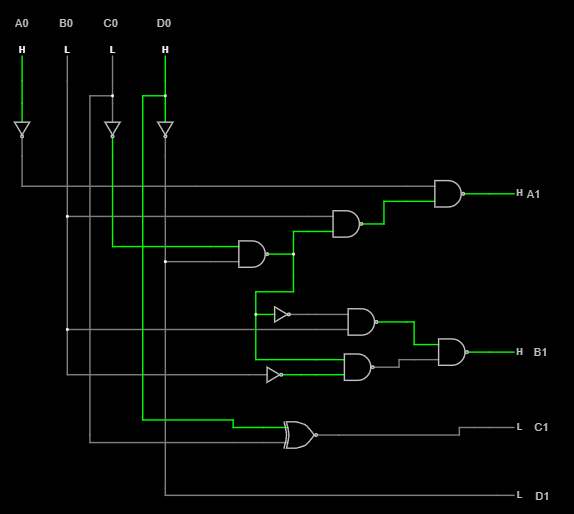
\includegraphics[width=0.7\textwidth]{Simplificacion1.png}
	\caption{Circuito final implementado con compuertas NAND, NOT y XNOR.}
	\label{fig:implementacion_nand_not}
\end{figure}


\begin{center}
	\href{\detokenize{https://www.falstad.com/circuit/circuitjs.html?ctz=DwYwlgTgBAZgvAIgIwKgFwM6IAwDpsEECsqYIiSeATAVQOx0DM2AHFQGwCcndqIARoiLZUAB0EJhqAG4QhqALaYhAUwC0SFAD4AUFCjAAMlAAeiFtigWrlpO1TwEIqKIoIA9Lv1HTFOuxsoJH8g+1gcDy8DYzMEeipA+NCHCM89aN8ERhYAFkDsvLsUpzE3NO8ASUzrJCoWRJznR2cMABscXBIoAAsweXKDKtik2vqkqkbilvanTtRe-qjgIcQCoLqoNYmmiKg2jq6FyUj05cyiEIuA9hZ6q6nUfdnDvuOBs9iidks6bDz2OgJX45B57GZ4F6LU4AOQAhgA7AAmmWBUBu9VulnRD3ecKR1U4AUYNCC2EBmxooIA9lDvHjkbF0ZtclYcvUCtTaQZ6Si-lAiJwEixCfzBZy3ksebE2ZYcmy0V8oHKWOKSLiEQzEJxagqApRyewvqqTt4AO7VSzWGp1HFLc2xazbfJ-W2ne3mSzMPLKzYu8Ild7uhA+r1WEVe11mzJMxg3IIhWMq-0iQOZYIBGoJm6RgxB3Lsln5zaxnPAPPyxixsNEkvJk256O3JUEXXNnYBu3RxWNLHdtmloPjRpQJI5Ip11PDcljgKj4kDzJzhIypXzied2JbYdrHLsEHrt2ZHd7pXWXf75r1stdgI+w23wkLxndkX3-k2g9R58BIgbK7vpNL0nIRLj-S5-CfRAmX-VF7k-BsHRFAUEm1BJkMghBUNFFCdT3dsUw3LVcPJTE0UBDDSIBIVrGxeDr0ZclUSYv0gMIhBUSo-kQiojD-04-84NYw9Yg41ggkFNFWAwpAJO+ep00kwDUjYhS5PjIlszooMvh+PkFOBaSQlRVSpK0o8WU0BJKz1WoMOsoIdXsix8KvIMnJbX8MQIDCRh1KgJgcqgfICyyRwClg1yE7wAFk0zJKySU0KtiRc95YtifUEjfJLriNOj0ooeKrDsByqxYccooMArkFYepCVsJAq3q6TaqgermTyZqzM3FlODlDq2u+OzC09CzbO61YxqsiyP0q+jECSR1yUsnzlr85bZuU4TCpIkrKGHcqwjm7SNiLfy8nzYKLuJMKLv7CashZc8Br6i8tq-IRTo806KvegwTC7KA1EYIg2ryYGgrrPZXgmVA0BURAAEECNOAGMoFIHGEKJtgZQKGMBh-d4cQAAhFHvDRhaiEYTHQbqGmIdBAmFqJhGEAAYXJ-6j3YAJgdBxgRUZ-HCbhtmABEueASnkDsTg2t+BzuAVxgmdF9AJZQd4Zc0AErCoGnNB4fWjt2Zm4lZxB2a1pYdbsa5DSV0HeaUkpoZZsXSZt1G0yQIgkApeXNGsStIcvd2Lc9hBEe97wAA14SpaBPgkiKgV-KxIr++bJFTkrPOK02O223OhXlAvLoeugM7T0kxLTlr65uyh69+4uPpq1u9T+S025R4B3HACBdCAA}}{Simplificación 1 en Falstad}
	\end{center}
	
	
	
	
	
	
	
	

	\section{Comparador Binario: Diseño, Simplificación, Simulación e Implementación}
	
	Para el segundo ejercicio se implementará un comparador binario de 2 bits. 
	El circuito tendrá cuatro entradas, de las cuales dos corresponden al número $A$ 
	y las otras dos al número $B$. Estas entradas se compararán para determinar 
	si $A$ es mayor que $B$, si $A$ es menor que $B$ o si ambos valores son iguales.
	
	Las entradas del comparador serán:
	
	\[
	A = A_1A_0
	\]
	
	\[
	B = B_1B_0
	\]
	
	Las salidas del circuito serán $S_0$, $S_1$ y $S_2$, las cuales indicarán las siguientes condiciones:
	
	\begin{itemize}
		\item $S_0$: indica que $A > B$.
		\item $S_1$: indica que $A < B$.
		\item $S_2$: indica que $A = B$.
	\end{itemize}
	
	Por lo tanto, el comportamiento esperado del comparador es el siguiente:
	
	\begin{enumerate}
		\item Si $A > B$:
		\[
		S_0 = 1 \quad \text{(LED encendido)}
		\]
		\[
		S_1 = 0 \quad \text{(LED apagado)}
		\]
		\[
		S_2 = 0 \quad \text{(LED apagado)}
		\]
		
		\item Si $A < B$:
		\[
		S_0 = 0 \quad \text{(LED apagado)}
		\]
		\[
		S_1 = 1 \quad \text{(LED encendido)}
		\]
		\[
		S_2 = 0 \quad \text{(LED apagado)}
		\]
		
		\item Si $A = B$:
		\[
		S_0 = 0 \quad \text{(LED apagado)}
		\]
		\[
		S_1 = 0 \quad \text{(LED apagado)}
		\]
		\[
		S_2 = 1 \quad \text{(LED encendido)}
		\]
	\end{enumerate}
	
	\subsubsection{Diseño}
	
	Como en el ejercicio anterior, para guiarnos mejor se realiza un diagrama en bloques 
	con sus respectivas entradas y salidas. Esto permite visualizar de manera más clara 
	el funcionamiento general del comparador antes de desarrollar la tabla de verdad, 
	las funciones lógicas y la implementación física.
	

	\begin{figure}[H]
		\centering
		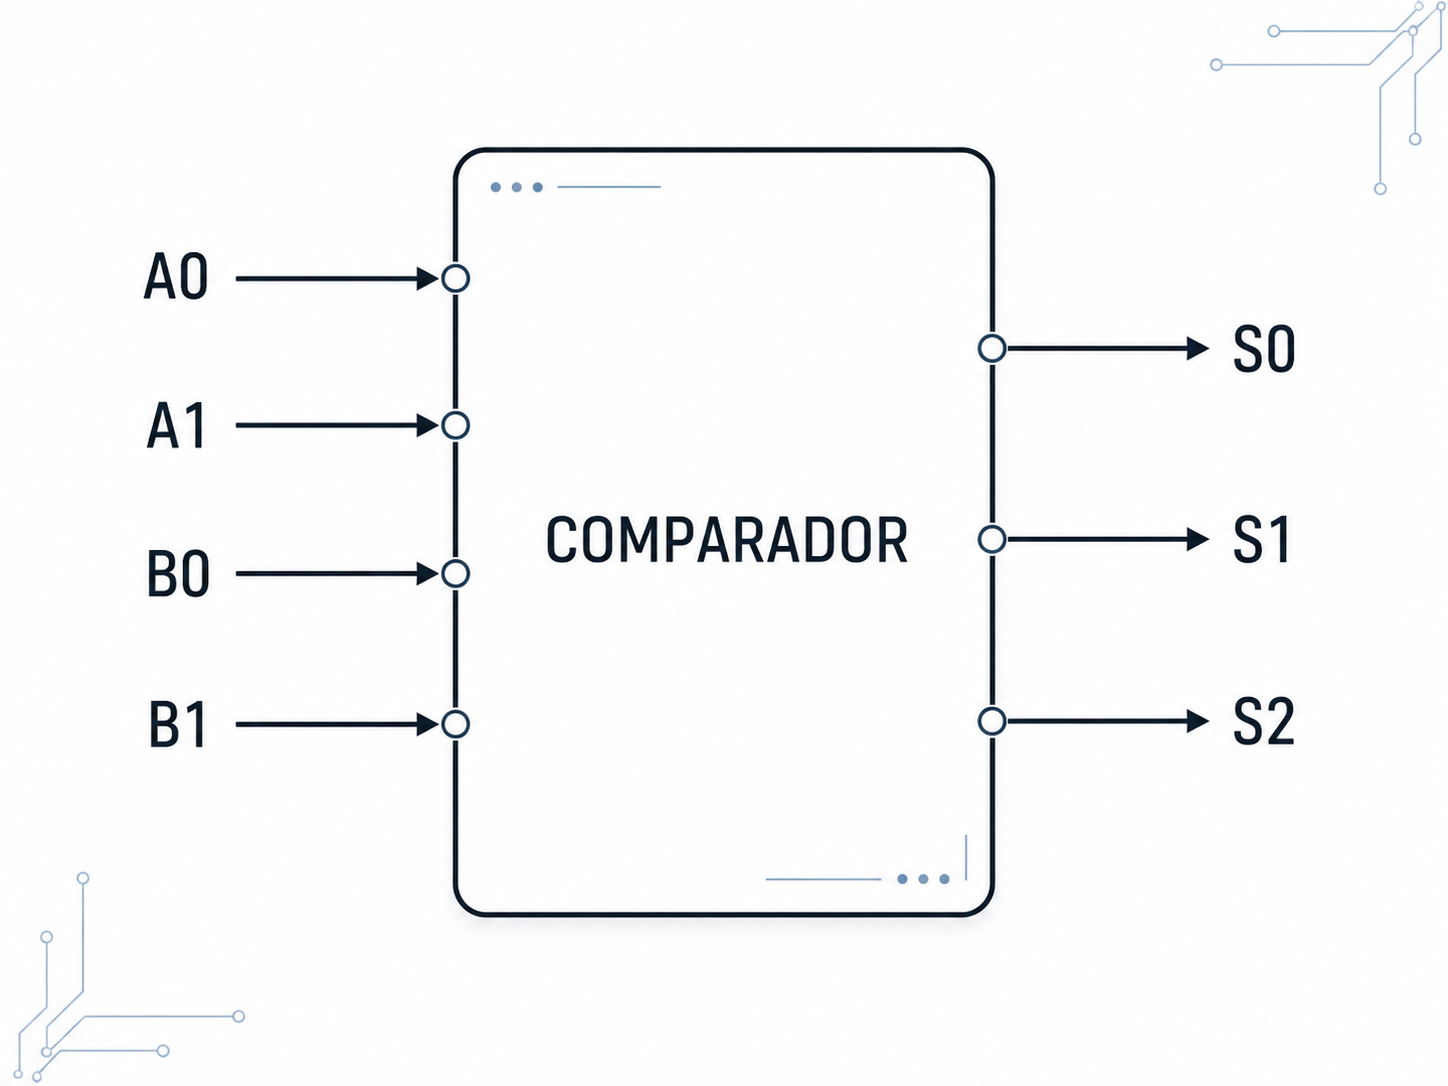
\includegraphics[width=0.3\textwidth]{Conversor2.png}
		\caption{Diagrama en bloques del comparador binario de 2 bits.}
		\label{fig:comparador_binario}
	\end{figure}
	
	
	
	\subsubsection{Tabla de verdad}
	
	La tabla de verdad muestra las distintas combinaciones posibles de las entradas 
	$A_0$, $A_1$, $B_0$ y $B_1$, junto con los valores correspondientes de las salidas 
	$S_1$, $S_2$ y $S_3$. Estas salidas indicarán si $A$ es mayor que $B$, si $A$ es menor 
	que $B$ o si ambos valores son iguales.
	
\[
\boxed{
	\begin{array}{c c|c c|c|c|c}
		A_1 & A_0 & B_1 & B_0 & S_0 & S_1 & S_2 \\ \hline
		0 & 0 & 0 & 0 & 0 & 0 & 1 \\
		0 & 0 & 0 & 1 & 0 & 1 & 0 \\
		0 & 0 & 1 & 0 & 0 & 1 & 0 \\
		0 & 0 & 1 & 1 & 0 & 1 & 0 \\ \hline
		
		0 & 1 & 0 & 0 & 1 & 0 & 0 \\
		0 & 1 & 0 & 1 & 0 & 0 & 1 \\
		0 & 1 & 1 & 0 & 0 & 1 & 0 \\
		0 & 1 & 1 & 1 & 0 & 1 & 0 \\ \hline
		
		1 & 0 & 0 & 0 & 1 & 0 & 0 \\
		1 & 0 & 0 & 1 & 1 & 0 & 0 \\
		1 & 0 & 1 & 0 & 0 & 0 & 1 \\
		1 & 0 & 1 & 1 & 0 & 1 & 0 \\ \hline
		
		1 & 1 & 0 & 0 & 1 & 0 & 0 \\
		1 & 1 & 0 & 1 & 1 & 0 & 0 \\
		1 & 1 & 1 & 0 & 1 & 0 & 0 \\
		1 & 1 & 1 & 1 & 0 & 0 & 1 \\
	\end{array}
}
\]
	
	\subsubsection{Simplificación}
	
	Luego de armar los mapas de Karnaugh, se obtienen las simplificaciones de las 
	funciones lógicas correspondientes a cada salida del comparador binario.

	
	

%---------------- MAPA S0 ----------------

\noindent
\begin{minipage}{0.62\textwidth}
	\[
	\begin{tikzpicture}
		
		\matrix (K) [kmap] {
			& 00 & 01 & 11 & 10 \\
			00 & 0 & 0 & 0 & 0 \\
			01 & 1 & 0 & 0 & 0 \\
			11 & 1 & 1 & 0 & 1 \\
			10 & 1 & 1 & 0 & 0 \\
		};
		
		\node[font=\scriptsize, above left=0.05cm and -0.15cm of K-2-1.north east] {$A_0A_1$};
		\node[font=\scriptsize, above right=0.02cm and -0.05cm of K-1-2.north west] {$B_0B_1$};
		
		\draw (K-2-1.north west) -- (K-1-2.south west);
		
		% Grupo verde
		\node[draw=green!60!black, grupo, fit=(K-3-2)(K-4-2)] {};
		
		% Grupo azul
		\node[draw=blue, grupo, fit=(K-4-2)(K-5-3)] {};
		
		% Grupo rojo
% Grupo rojo abierto a la derecha y separado de la celda
\draw[red, line width=1.2pt, rounded corners]
([xshift=1pt,yshift=-1pt]K-4-5.north east) --
([xshift=-1pt,yshift=-1pt]K-4-5.north west) --
([xshift=-1pt,yshift=1pt]K-4-5.south west) --
([xshift=1pt,yshift=1pt]K-4-5.south east);
		
	\end{tikzpicture}
	\]
\end{minipage}
\hfill
\begin{minipage}{0.33\textwidth}
\[
S_0 = A_0\overline{B_0} + A_1\overline{B_1}(\overline{B_0} + A_0)
\]
\end{minipage}

\vspace{1cm}

%---------------- MAPA S1 ----------------

\noindent
\begin{minipage}{0.62\textwidth}
	\[
	\begin{tikzpicture}
		
		\matrix (K) [kmap] {
			& 00 & 01 & 11 & 10 \\
			00 & 0 & 1 & 1 & 1 \\
			01 & 0 & 0 & 0 & 1 \\
			11 & 0 & 0 & 0 & 0 \\
			10 & 0 & 0 & 1 & 0 \\
		};
		
		\node[font=\scriptsize, above left=0.05cm and -0.15cm of K-2-1.north east] {$A_0A_1$};
		\node[font=\scriptsize, above right=0.02cm and -0.05cm of K-1-2.north west] {$B_0B_1$};
		
		\draw (K-2-1.north west) -- (K-1-2.south west);
		
		% Grupo verde
		\node[draw=green!60!black, grupo, fit=(K-2-3)(K-2-4)] {};
		
		% Grupo azul
		\node[draw=blue, grupo, fit=(K-2-4)(K-3-5)] {};
		
		% Grupo rojo
% Grupo rojo abierto abajo y separado de la celda
\draw[red, line width=1.2pt, rounded corners]
([xshift=-1pt,yshift=1pt]K-5-4.south west) --
([xshift=-1pt,yshift=-1pt]K-5-4.north west) --
([xshift=1pt,yshift=-1pt]K-5-4.north east) --
([xshift=1pt,yshift=1pt]K-5-4.south east);
	\end{tikzpicture}
	\]
\end{minipage}
\hfill
\begin{minipage}{0.33\textwidth}
	\[
	S_1 = \overline{A_0}B_0 + \overline{A_1}B_1(\overline{A_0} + B_0)
	\]
\end{minipage}

\vspace{1cm}

%---------------- MAPA S2 ----------------

\noindent
\begin{minipage}{0.62\textwidth}
	\[
	\begin{tikzpicture}
		
		\matrix (K) [kmap] {
			& 00 & 01 & 11 & 10 \\
			00 & 1 & 0 & 0 & 0 \\
			01 & 0 & 1 & 0 & 0 \\
			11 & 0 & 0 & 1 & 0 \\
			10 & 0 & 0 & 0 & 1 \\
		};
		
		\node[font=\scriptsize, above left=0.05cm and -0.15cm of K-2-1.north east] {$A_0A_1$};
		\node[font=\scriptsize, above right=0.02cm and -0.05cm of K-1-2.north west] {$B_0B_1$};
		
		\draw (K-2-1.north west) -- (K-1-2.south west);
		
	\end{tikzpicture}
	\]
\end{minipage}
\hfill
\begin{minipage}{0.33\textwidth}
	Función impar, por lo tanto no se puede simplificar:
	
\[
\begin{aligned}
	S_2 ={}& \overline{A_0}\,\overline{A_1}\,\overline{B_0}\,\overline{B_1} \\
	&+ \overline{A_0}A_1\overline{B_0}B_1 \\
	&+ A_0A_1B_0B_1 \\
	&+ A_0\overline{A_1}B_0\overline{B_1}
\end{aligned}
\]
\end{minipage}
	
	\newpage

	\subsubsection{Simulación}
	
	Luego de obtener las funciones lógicas del comparador binario, se realizó la simulación
	del circuito para verificar su correcto funcionamiento. En la siguiente figura se puede
	observar el circuito implementado en el simulador.
	
	\begin{figure}[H]
		\centering
		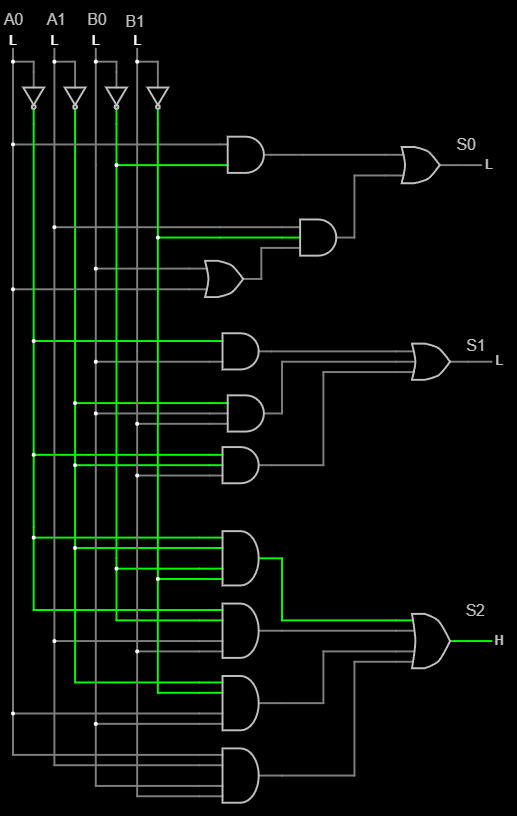
\includegraphics[width=0.55\textwidth]{Compuertas2.png}
		\caption{Simulación del comparador binario de 2 bits.}
		\label{fig:simulacion_comparador}
	\end{figure}
	\begin{center}
		\href{\detokenize{https://falstad.com/circuit/circuitjs.html?ctz=DwYwlgTgBAZgvAIgIwKgFwM6IAwDpsEECsqYIiSeATAVQOx0DM2AHFQGwCcndqIARoiLZUAB0EJhqAG4QhqALaYhAUwC0SFAD4AUFCjAAHlENDsUIuyh1OFzqngIALKgxhEVF+hWIAgiIB6XX0jEwobCysaFjsHRC83Dy80HwQAIUDgg2NTZCQrSygkJyJY2HjXdwRPVBS-FCC9bLDqxhiiGI46KHYUcudKpNrUtIas4AAZFvYnIqQqHtmWEX7MpsmW+ZjNBa2oZbiENZCp3KROXfmii-2Vx2ODU49CnagqQoPVhEaQgEkWzhWPaAt6sQ4rDAAGxwuBIUAAFlUSD8DP8zuxzHt8uZouDXNCjrDUIj5CjgGiPJ4ilROlTcV8oFCYXCSZJvuMKdUWNsaW9uaCWHjGQS8Cykez1gB3aazV4gnZ4snS3Ly3ny+aK8bKii817YuZUTVSzYY6nbU0Kr5KzY3V5UKmW+4SkLa6oO3n22Uaq1alrvIFXGnbb1O625INmvnBw0+9YAeWguRmOLoCzoRAW9Bjod9Z1tV3OmdTRpdfpegcKnjuOGdBgAsi100WFssU9ma2Scoh0zinLYGLZ3u2BoyqjVvIgAMoPYC+AB2ABMWk5llA2rMiDd10KwHPEIxa8AEy1GIwrE4V1ALzFryWDPOl7l129Ck4Zi-2Hej4nEOxCkQ6CsQD2kAnc9wQA8w2eKInBxf8MS-V19WiIpTQzQVYxCBtcmAixAP2fI8M-TDmhwv8LE3axOA3dhhwSMdklSScxnWbDu3YbYCBiFhCMoMESNCMjZh4cwbEYKAeAPfp6KGCcEEnQ0oIglhZirRY3lgxCTxUt5UzeOliwE1131ed8qy08M6VYfTVMMnNjVyN9VP-CtiPskIHxPDjInMJyfIsnVo0jM8MPcgwkN5EK1x0kKAq5TprIjbcjO02ZnySlS4qIVzFjgtyO1zfcYu8ldzFilKnxinTSuirwwuAV0atg3zL2auLryvAgr1alc4sLXTdhuJxGGHGckKGka1zPK8RriszYPUpy5tmPzT3PGYsq3HTN0zblNt2mJkyjdr30scw-wKBCKsQEEUJBIgLzi+6LzXbyHrqgqHIoCbBoWAD8qOQ9xr+-Cov+r9PKfbyLqvVcLrA-cgZNcx0NQ87NOu5BTSOqLkz6m5-uuBZ4cx-qYdxyw4v9HyPx6OzPtLcNCnYPTcfpwGlJqmGavBzGefwmHefqyH928ph1tmcWEYgpGVQKF6QVTasOcKhBFZoV6YiVvrsYW-UpdJ01xc16wzyp5m9OpptzaAjMTetvn32N97TYBsaWhd52Xp2rLvZuQWLi-Y8kxeLjrG8vjQprKBdwqKAAHtSXGEWILt7lfNXdPpa8RO2TJFPGDt7gFhq4vs8PAu7c0bAVtXauPsBmPwJcfPFxPKuqEImr5nyculPV8wQRYWbDdE6b9RYDbMc9AabP2T56tdDLVP5TgQwZ8K-VXq5C4WNfRtl-c09uqkWEBOLd-2EzTUnhv3afNPLyH3rMefmIh5Hxe-VPk+lgXjeGoAisCpd+VhATK3vpSJYv8JKgUxpfHgUQqSIIvkXU0IJwF9UihHXUXFUG7DDliPB09ChNlppQccX8H4ELpKHShACkI32vpibA7NIHxQkoGfklA9rwKrqw3YFoBFU24awGIl8eFRxVl9BA74-ImUoHfQ+yB-YvHzGbPhlxx7qLdsoiR8x0YGggcohRNd1I7GMUpfROkFGZUxrY2YCiaBYM4tZLENBLGqwkR4yMBjPEyP6pobRuwqCfwYe3EJk1AmhIPkpamFDnJAk8FI9h3jLzxOSe1OuncCi2hyftakhEdpFBrv4xmQhbSlJ6KHDGVDfx0I3C9BJWTMSKIsE0xRvsvRmJds0+xhRi6w0HoHfpYD8KlzgXU5wq5EFDPnv44AARwAQF0EAA}}{Simulación 2 en Falstad}
	\end{center}
	
	
	
	Como se puede observar en la simulación, las entradas se encuentran en el siguiente estado:
	
	\[
	A_0 = 0,\quad A_1 = 0,\quad B_0 = 0,\quad B_1 = 0
	\]
	
	Por lo tanto, los valores de entrada corresponden a:
	
	\[
	A = 00
	\]
	
	\[
	B = 00
	\]
	
	En este caso se cumple que:
	
	\[
	A = B
	\]
	
	Por este motivo, las salidas del comparador toman los siguientes valores:
	
	\[
	S_0 = 0,\quad S_1 = 0,\quad S_2 = 1
	\]
	
	Esto coincide con lo indicado en la tabla de verdad, ya que cuando ambos números son
	iguales, solamente debe activarse la salida correspondiente a la igualdad. La simulación
	del circuito puede observarse en el enlace correspondiente a la Simulación 2.
	
	\subsubsection{Implementación}
	
	Una vez verificado el funcionamiento mediante la simulación, se pasa a la implementación
	física del circuito utilizando compuertas lógicas y LEDs indicadores. Al igual que en el
	ejercicio anterior, cada salida del comparador se conecta a un LED para comprobar
	visualmente el estado lógico de cada condición.
	
	Para facilitar la implementación física del circuito, se utilizarán compuertas lógicas
	equivalentes a las funciones simplificadas obtenidas mediante los mapas de Karnaugh.
	De esta manera, el circuito permitirá indicar si $A$ es mayor que $B$, si $A$ es menor
	que $B$ o si ambos valores son iguales.

	
	\subsubsection{Implementación con compuertas NAND y NOT}
	
	Para la implementación física del comparador, se procede a transformar las funciones
	lógicas obtenidas a compuertas NAND y NOT.
	
	\paragraph{Para $S_0$:}
	
	\[
	S_0 = A_0\overline{B_0} + A_1\overline{B_1}(\overline{B_0} + A_0)
	\]
	
	\[
	S_0 = A_0\overline{B_0} + A_1\overline{B_1}\cdot \overline{\overline{(\overline{B_0} + A_0)}}
	\]
	
	\[
	S_0 = A_0\overline{B_0} + A_1\overline{B_1}\cdot
	\overline{(B_0 \cdot \overline{A_0})}
	\]
	
	\[
	S_0 =
	\overline{
		\overline{
			A_0\overline{B_0} + A_1\overline{B_1}\cdot
			\overline{(B_0 \cdot \overline{A_0})}
		}
	}
	\]
	
	\[
	S_0 =
	\overline{
		\overline{A_0\overline{B_0}}
		\cdot
		\overline{
			A_1\overline{B_1}\cdot
			\overline{(B_0 \cdot \overline{A_0})}
		}
	}
	\]
	
	\paragraph{Para $S_1$:}
	
	\[
	S_1 = \overline{A_0}B_0 + \overline{A_1}B_1(\overline{A_0} + B_0)
	\]
	
	\[
	S_1 = \overline{A_0}B_0 + \overline{A_1}B_1\cdot
	\overline{\overline{(\overline{A_0} + B_0)}}
	\]
	
	\[
	S_1 = \overline{A_0}B_0 + \overline{A_1}B_1\cdot
	\overline{(A_0 \cdot \overline{B_0})}
	\]
	
	\[
	S_1 =
	\overline{
		\overline{
			\overline{A_0}B_0 + \overline{A_1}B_1\cdot
			\overline{(A_0 \cdot \overline{B_0})}
		}
	}
	\]
	
	\[
	S_1 =
	\overline{
		\overline{\overline{A_0}B_0}
		\cdot
		\overline{
			\overline{A_1}B_1\cdot
			\overline{(A_0 \cdot \overline{B_0})}
		}
	}
	\]
	
	\paragraph{Para $S_2$:}
	
	Para la salida $S_2$, se observa que corresponde al caso en el que ambos números son
	iguales. Por lo tanto, se puede aprovechar la comparación bit a bit mediante compuertas
	XNOR:
	
\[
S_2 = S_0 \odot S_1
\]
	
	donde el símbolo $\odot$ representa la operación XNOR.
	
	
	
	
	\subsubsection{Circuito a implementar}
	
	\begin{figure}[h]
		\centering
		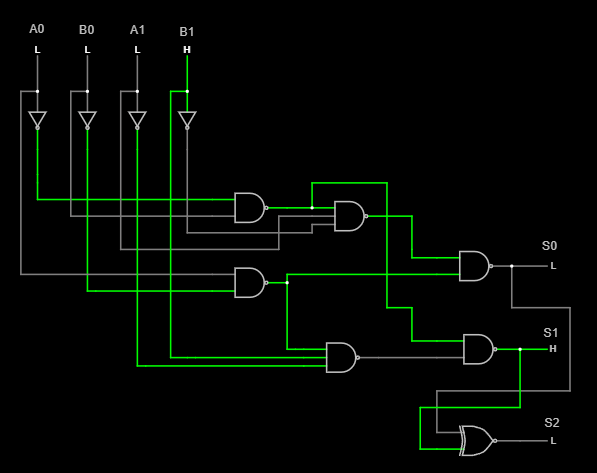
\includegraphics[width=0.7\textwidth]{Simplificacion2.png}
		\caption{Circuito final implementado con compuertas NAND, NOT y XNOR.}
		\label{fig:implementacion_nand_not}
	\end{figure}
	
	
	
	\begin{center}
		\href{\detokenize{https://www.falstad.com/circuit/circuitjs.html?ctz=DwYwlgTgBAZgvAIgIwKgFwM6IAwDpsEECsqYIiSeATAVQOx0DM2AHFQGwCcndqIARoiLZUAB0EJhqAG4QhqALaYhAUwC0SFAD4AUFCjAAMlAAeiFtihI67KBaid2qeAhEB6XfqOmKNq3+tbR2ccBA89A2MzBHoqf1tYhydYUPCvKMRGdhZ4qCyc4JTXMQowzwMTHwR2ABYoWodGet4ikSgMMEQqGtQ0FUQAQXdy4EropHZLdlskFk56zhDi9s6YnvR+hAAhYYjRqsYiJrpLRjYoJiW2jq71vsQtlDSKqqoiHOmoKhY6BavUG5rXqbAZPEYASSq9kCdks3xY-3aABscLgSFAABarEjPYCQ6L5XKE+GIjAo1xo1BY+S4-FdOhxGGJEmtAHkvDo6mSMp7AByAEMAHYAEyqkxyNQmFyIcUlyRcbTAgsyqAA9jSRgKRVU5VAagQoERJnqCIj1dzcVrRdFdUQanUjZY7esFWqNXyhdbzDUckQkHFuHE-VR-pbPVCfc1GQQPgyze6vFaqkROHFsjkmLZ04ilSraVUYYW-CzXcjUZzsTyvAANQWq6DRFiRps5SisOw+0MjACyVUDhv9VmwDIHIdZuN74xjUaHI-YcfHPYL05bs7iLa7ewA7lC4SwcvZGFlN14d43TllYXkZSeDGfEHQZXqpRZLHLb8B7whX8-bD+fW0rq4l+-72P+hRASMIEGjUjgdhKEGpFBu5TEa8H1EaH4QNB16ylKZwuqEWgWAANIcVAANykQRFFymRTbAG42EjNhybGvqUzthx-xaI6JEcRR4r8QQjHMduYpcVKzq-h+X7Sba9p6hYsnJopAFfPqSmAUh4nRIkTKaYEKl6YZxaaQBxmZNkXz7nk1n2gii66VZEqRuKeqdk5p4SRKjBplxnmQc5CC6rqSBqRMlnIAEASKUZXl3gWcWxXU74JZ+Ea+t8hrGjKjlBd50SOoa2XFc6UW2saSCpjl2nFMBBbFrZMKOlF1VBlVfitelX62tlkZ5VF0J+JG8UFYlNqtiNWX5TphVCDV85Bn4S1RWVinFatPVsVMI5ECtC7jRl0SZvUtmrtm21FYttkEWds31chBLWemeRNvdUXMrZiQnIRj3BSmcS-TZGbYH9uzzTEtnAz9YNRf2wYODVgPw8jNWaGDhqpm1lAOujuPSmOR1fhjdSPuukbk0NlNPquLB+W105LUO7Z0E2jOs+9LBSmz4NVhN5g81zL61ENIt1HTotXS5RKXmNc0CwgR4zH4ysfdLSuXq9hKXcTKEYX+Booxr7kcfU7bkVF7nkYTuFReTuG28besnU+gOwk62PpWMFDYMISnRnQ8w+uipaAt0wKIAAyhDLxTkc9SjawaZ+qSqwRxs0dgnsPvIH7RB2FQ0Zc28ae3JHCBRyG4SMeAEC6EAA}}{Simplificación 2 en Falstad}
	\end{center}
	
	
	
	
	\newpage
	\clearpage
	\phantomsection
	\addcontentsline{toc}{section}{Bibliografía}
	\begin{thebibliography}{9}
		
		\bibitem{simulacion1}
		Simulación 1: Conversor BCD a Exceso-3. Disponible en:
		\url{https://tinyurl.com/27fbgv4n}
		
		\bibitem{simplificacion1}
		Simplificación 1: Conversor BCD a Exceso-3. Disponible en:
		\url{https://tinyurl.com/263xffme}
		
		\bibitem{simulacion2}
		Simulación 2: Comparador binario. Disponible en:
		\url{https://tinyurl.com/26u3vja8}
		
		\bibitem{simplificacion2}
		Simplificación 2: Comparador binario. Disponible en:
		\url{https://tinyurl.com/2cpp9ej3}
		
	\end{thebibliography}
	
\end{document}